\subsection{Escenaris de prova i resultats}
\label{sec:escenaris_resultats}

Els escenaris següents s’han dissenyat per exercitar els patrons de transacció més rellevants implementats al prototip. Cada prova inclou el seu objectiu, els requisits associats, la preparació necessària, el resultat esperat i l’evidència que s’ha de recollir.

\subsubsection{Escenari A -- Interceptació bàsica i visualització dins de MetaMask}

\noindent\textbf{Objectiu.} Verificar que MetaMask Flask invoca correctament el Snap abans de la confirmació d’una transacció.

\noindent\textbf{Requisits validats.} RF1, RF4 i parcialment RNF3.

\noindent\textbf{Preparació.} S’inicia una transacció des de la DApp local amb MetaMask Flask, el Snap i el backend en execució.

\noindent\textbf{Resultat esperat.} El Snap ha d’interceptar la transacció, enviar-ne les dades al backend i mostrar un \textit{insight} dins de MetaMask abans de la confirmació final.

\noindent\textbf{Resultat observat.} Les deu repeticions automatitzades del cas A1 van produir deu vertaders negatius amb risc \texttt{BAJO}, puntuació 10 i acció \texttt{ALLOW}. En la validació d'interfície, MetaMask va activar el Snap abans de la confirmació i va mostrar el mateix resultat. L'execució manual va quedar registrada a SQLite amb l'identificador 43. La primera captura es va obtenir accidentalment a \textit{mainnet}; el flux sobre Sepolia es va confirmar posteriorment a l'escenari G.

\noindent\textbf{Evidència.} Captura de MetaMask amb l’\textit{insight} visible (Figura~\ref{fig:eval_scenario_a}), registre del backend i resposta JSON generada.

\begin{figure}[htbp]
    \centering
    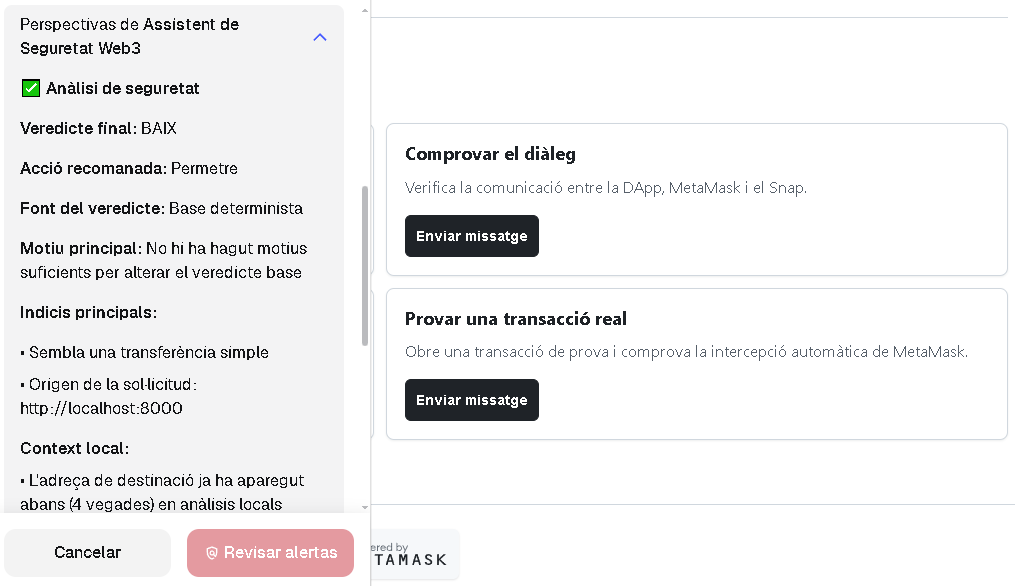
\includegraphics[width=0.48\textwidth]{imgs/eval_scenario_a.png}
    \caption{Insight del Snap mostrat abans de confirmar la transacció}
    \label{fig:eval_scenario_a}
\end{figure}



\subsubsection{Escenari B -- Aprovació ERC20 limitada i revocació}

\noindent\textbf{Objectiu.} Comprovar que el sistema diferencia una aprovació limitada d’una revocació de permisos mitjançant una quantitat igual a zero.

\noindent\textbf{Requisits validats.} RF2, RF3 i RF4.

\noindent\textbf{Preparació.} S’executen dues operacions ERC20: una aprovació limitada mitjançant \texttt{approve(spender, amount)} i una revocació mitjançant \texttt{approve(spender, 0)}.

\noindent\textbf{Resultat esperat.} El sistema ha d’identificar el tipus d’operació, indicar el destinatari del permís i classificar la revocació com una operació de risc baix. L’aprovació limitada ha de rebre un tractament menys restrictiu que una aprovació il·limitada.

\noindent\textbf{Resultat observat.} Les deu repeticions de B1 van identificar \texttt{approve}\allowbreak\texttt{(address,uint256)} amb una quantitat de $10^{18}$ unitats com una aprovació limitada: risc \texttt{BAJO}, puntuació 20 i \texttt{ALLOW}. Les deu repeticions de B2, amb quantitat zero, es van descriure com una revocació i van obtenir risc \texttt{BAJO}, puntuació 5 i \texttt{ALLOW}. Els registres manuals de referència corresponen als identificadors 36 i 37; una comprovació des d'Etherscan Sepolia va quedar registrada amb l'identificador 45.

\noindent\textbf{Evidència.} Captures dels \textit{insights} (Figura~\ref{fig:eval_scenario_b}), dades descodificades de la transacció i registres del motor de regles.

\begin{figure}[htbp]
    \centering
    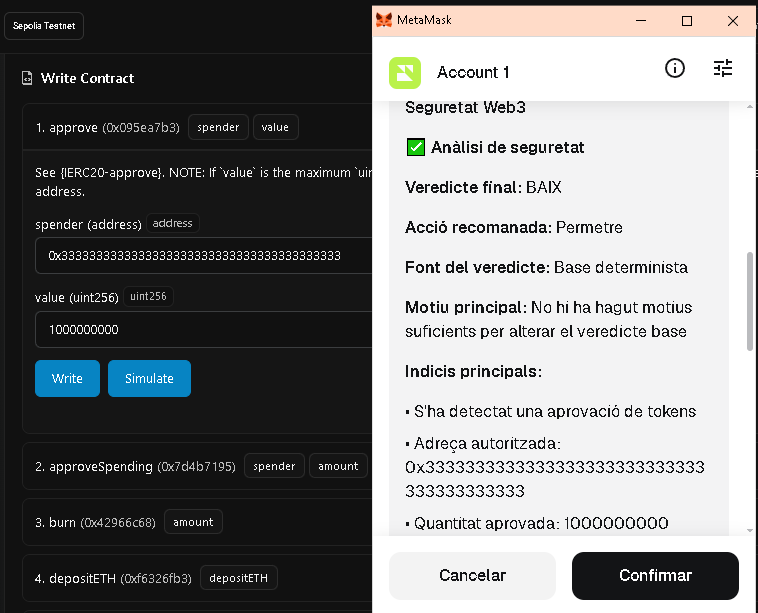
\includegraphics[width=0.48\textwidth]{imgs/eval_scenario_b.png}
    \caption{Detecció d'una aprovació ERC20 limitada iniciada des d'Etherscan}
    \label{fig:eval_scenario_b}
\end{figure}



\subsubsection{Escenari C -- Aprovació ERC20 pràcticament il·limitada}

\noindent\textbf{Objectiu.} Verificar la detecció d’una aprovació ERC20 amb una quantitat màxima o pràcticament il·limitada.

\noindent\textbf{Requisits validats.} RF2, RF3 i RF4.

\noindent\textbf{Preparació.} S’executa una operació \texttt{approve(spender, MaxUint256)} o una quantitat equivalentment elevada sobre el contracte de proves.

\noindent\textbf{Resultat esperat.} El backend ha d’identificar l’aprovació com a il·limitada, assignar un nivell de risc alt i recomanar una revisió abans de confirmar la transacció.

\noindent\textbf{Resultat observat.} Les deu repeticions de C1 van descodificar \texttt{MaxUint256} com una aprovació il·limitada i van obtenir risc \texttt{ALTO}, puntuació 90 i recomanació \texttt{REVIEW}. El motor determinista va mantenir prioritat sobre la revisió de la IA. Una execució manual de referència es conserva al registre 38.

\noindent\textbf{Evidència.} Captura de MetaMask (Figura~\ref{fig:eval_scenario_c}), resposta estructurada del backend, indicis generats i informació descodificada de la transacció.

\begin{figure}[H]
    \centering
    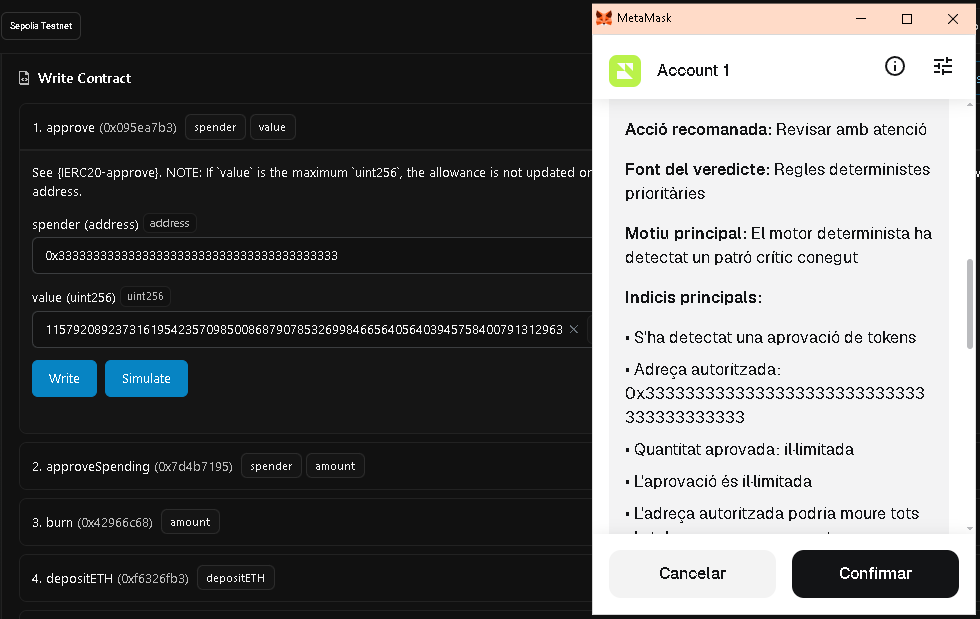
\includegraphics[width=0.94\textwidth]{imgs/eval_scenario_c.png}
    \caption{Aprovació ERC20 amb \texttt{MaxUint256} classificada com a risc alt abans de confirmar-la}
    \label{fig:eval_scenario_c}
\end{figure}



\subsubsection{Escenari D -- Permís global ERC721 sobre NFTs}

\noindent\textbf{Objectiu.} Comprovar la detecció d’un permís global sobre una col·lecció NFT i diferenciar-lo d’una revocació posterior.

\noindent\textbf{Requisits validats.} RF2, RF3 i RF4.

\noindent\textbf{Preparació.} S’executen dues operacions sobre el contracte ERC721 de proves: \texttt{setApprovalForAll(operator, true)} i \texttt{setApprovalForAll(operator, false)}.

\noindent\textbf{Resultat esperat.} L’activació del permís global ha de ser identificada com una operació d’alt risc, ja que l’operador podria gestionar tots els NFTs de la col·lecció. La revocació ha de ser descrita com una acció de risc baix.

\noindent\textbf{Resultat observat.} Les deu repeticions de l'activació del permís global (D1) van obtenir risc \texttt{ALTO}, puntuació 95 i \texttt{REVIEW}; les deu repeticions de la revocació (D2) van obtenir risc \texttt{BAJO}, puntuació 5 i \texttt{ALLOW}. Les execucions manuals de referència corresponen als registres 39 i 40.

\noindent\textbf{Evidència.} Captures de MetaMask per als dos sentits del permís (Figura~\ref{fig:eval_scenario_d}), dades descodificades, indicis generats i resposta final del backend.

\begin{figure}[H]
    \centering
    \begin{subfigure}[t]{0.49\textwidth}
        \centering
        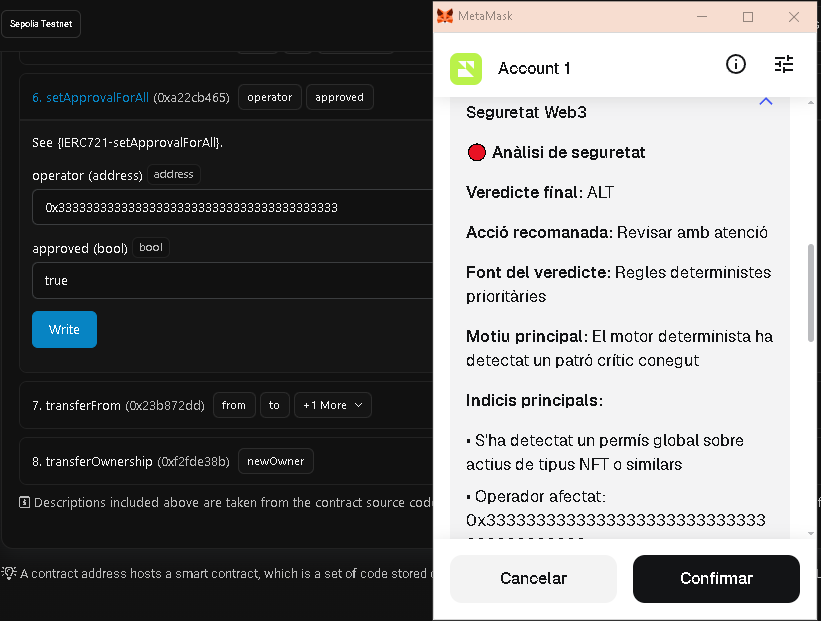
\includegraphics[width=\textwidth]{imgs/eval_scenario_d1.png}
        \caption{Activació del permís global: risc \texttt{ALTO}}
        \label{fig:eval_scenario_d1}
    \end{subfigure}\hfill
    \begin{subfigure}[t]{0.47\textwidth}
        \centering
        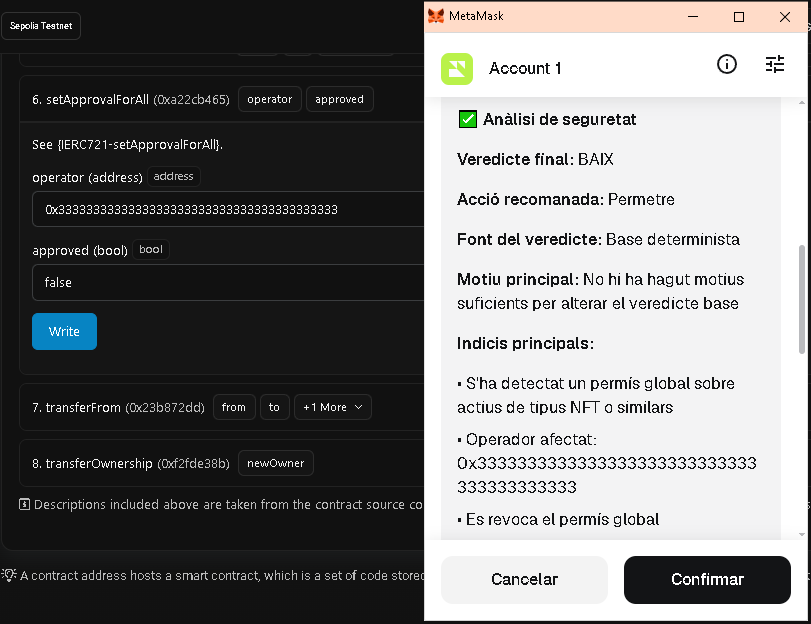
\includegraphics[width=\textwidth]{imgs/eval_scenario_d2.png}
        \caption{Revocació del permís: risc \texttt{BAJO}}
        \label{fig:eval_scenario_d2}
    \end{subfigure}
    \caption[Diferenciació entre l'activació i la revocació d'un permís global ERC721]{Diferenciació de \texttt{setApprovalForAll(true)} i \texttt{setApprovalForAll(false)} sobre el contracte NFT de Sepolia}
    \label{fig:eval_scenario_d}
\end{figure}



\subsubsection{Escenari E -- Context local i adreces etiquetades}

\noindent\textbf{Objectiu.} Verificar que el sistema incorpora informació procedent de la base de dades local i de les etiquetes d’adreces conegudes dins del veredicte.

\noindent\textbf{Requisits validats.} RF2, RF3, RNF2 i RNF4.

\noindent\textbf{Preparació.} S’analitza una transacció dirigida a una adreça registrada prèviament a la base de dades o etiquetada per una font externa com a adreça de risc.

\noindent\textbf{Resultat esperat.} El backend ha d’afegir context rellevant sobre l’adreça, reflectir-lo en els indicis i evitar que aquest context es presenti com una prova absoluta si només constitueix una alerta informativa.

\noindent\textbf{Resultat observat.} Es va registrar una adreça controlada amb l'etiqueta \texttt{scam}. Les deu repeticions d'E1 van incorporar aquesta condició, van aplicar l'ajust de context i van obtenir risc \texttt{ALTO} amb puntuació 60. Una execució manual que inclou la coincidència i la font als indicis es conserva al registre 41.

\noindent\textbf{Evidència.} Registres de SQLite, coincidències amb etiquetes conegudes, resposta JSON i captura de l’\textit{insight} mostrat a MetaMask (Figura~\ref{fig:eval_scenario_e}).

\begin{figure}[H]
    \centering
    \begin{subfigure}[t]{0.37\textwidth}
        \centering
        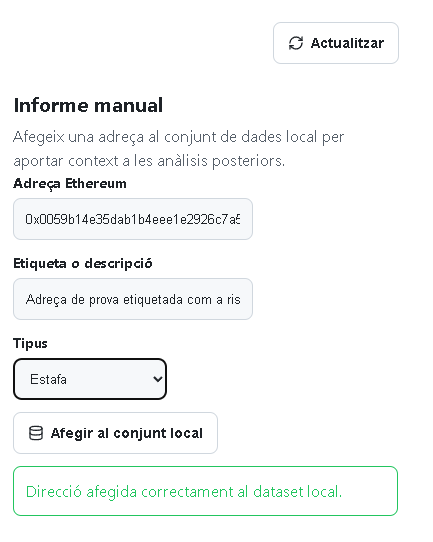
\includegraphics[width=\textwidth]{imgs/eval_scenario_e_report.png}
        \caption{Alta manual de l'adreça controlada amb tipus \texttt{scam}}
        \label{fig:eval_scenario_e_report}
    \end{subfigure}\hfill
    \begin{subfigure}[t]{0.59\textwidth}
        \centering
        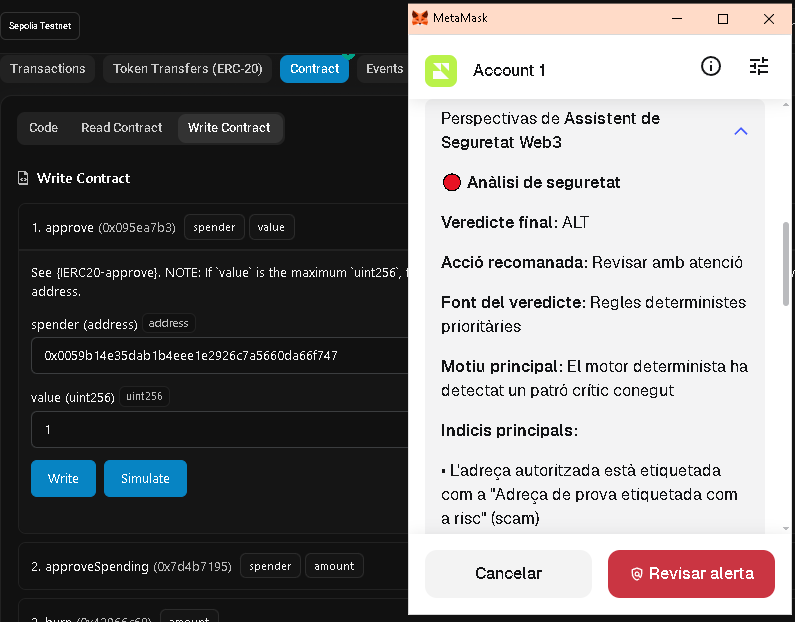
\includegraphics[width=\textwidth]{imgs/eval_scenario_e.png}
        \caption{Aprovació limitada elevada a risc \texttt{ALTO} pel context de l'adreça}
        \label{fig:eval_scenario_e_result}
    \end{subfigure}
    \caption{Incorporació d'una etiqueta local de risc al veredicte de l'escenari E}
    \label{fig:eval_scenario_e}
\end{figure}



\subsubsection{Escenari F -- Explicació de la IA i control semàntic}

\noindent\textbf{Objectiu.} Avaluar si la IA genera explicacions comprensibles i comprovar que la capa de control semàntic evita afirmacions incompatibles amb els fets detectats.

\noindent\textbf{Requisits validats.} RF3, RNF4 i RNF5.

\noindent\textbf{Preparació.} S’analitzen transaccions representatives dels escenaris anteriors i es comparen les explicacions generades amb els fets tècnics confirmats pel motor de regles.

\noindent\textbf{Resultat esperat.} L’explicació ha d’indicar correctament el tipus d’operació i el risc associat. No ha de mencionar aprovacions il·limitades, permisos globals, enviament d’ETH o adreces malicioses quan aquests elements no estiguin presents a la transacció analitzada.

\noindent\textbf{Resultat observat.} El pilot inicial amb Ollama va revelar que el model proposava \texttt{ALTO} fins i tot per transferències simples i revocacions, fet que generava quatre falsos positius. Es va reforçar el control semàntic perquè una IA complementària no pugui elevar un risc \texttt{BAJO} sense una aprovació il·limitada, un permís global actiu o una etiqueta objectiva de risc. També es va ampliar el sanejament després de detectar una referència inventada a un permís de tokens en una transferència simple. En la revisió visual final va aparèixer una nova variant, \textit{``Se permite mover tokens''}, que expressava la mateixa autorització inexistent sense utilitzar la paraula \textit{permiso}. Es van afegir variants semàntiques equivalents a la regla i una prova de regressió. Després de reiniciar els serveis, la mateixa operació va conservar el veredicte \texttt{BAJO} i va generar una explicació local segura: una transferència simple sense permisos de tokens. Les 80 observacions automatitzades van permetre confirmar la consistència dels patrons principals i detectar, separadament, el límit de classificació documentat al cas C2.

\noindent\textbf{Evidència.} Prompts, respostes d’Ollama, camps \texttt{ai\_review}, explicació final i resultats de la capa de sanejament semàntic, amb la comparació abans i després a la Figura~\ref{fig:eval_scenario_f}.

\begin{figure}[H]
    \centering
    \begin{subfigure}[t]{0.48\textwidth}
        \centering
        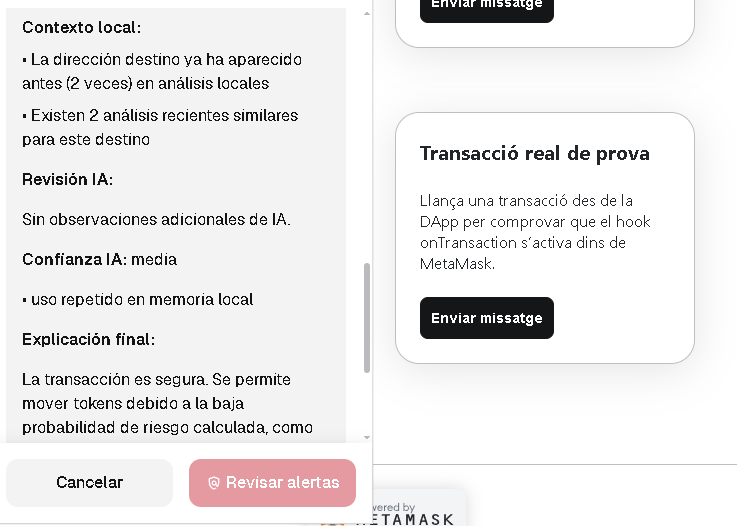
\includegraphics[width=\textwidth]{imgs/eval_scenario_f_before.png}
        \caption{Abans: autorització de tokens inventada per la IA}
        \label{fig:eval_scenario_f_before}
    \end{subfigure}\hfill
    \begin{subfigure}[t]{0.48\textwidth}
        \centering
        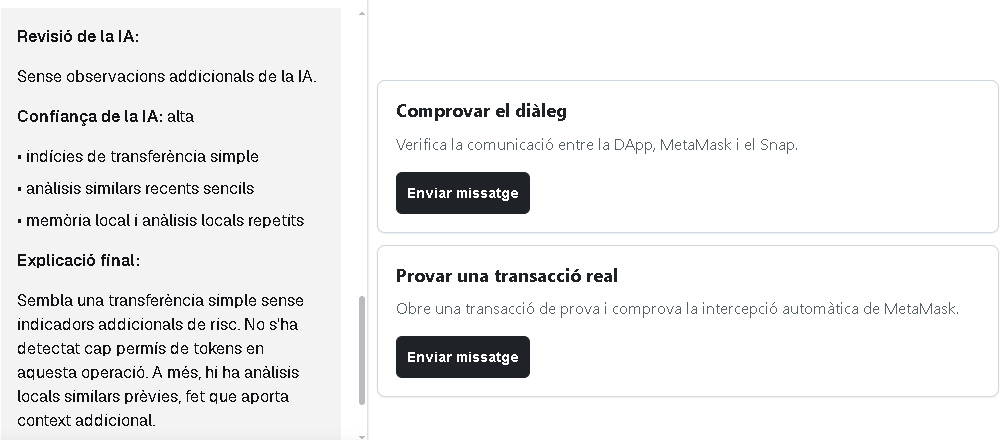
\includegraphics[width=\textwidth]{imgs/eval_scenario_f.png}
        \caption{Després: explicació local coherent amb els fets}
        \label{fig:eval_scenario_f_after}
    \end{subfigure}
    \caption{Validació del sanejament semàntic aplicat a una transferència simple}
    \label{fig:eval_scenario_f}
\end{figure}



\subsubsection{Escenari G -- Flux complet sobre Sepolia i Etherscan}

\noindent\textbf{Objectiu.} Validar el recorregut complet del sistema sobre una transacció real generada des d’Etherscan i dirigida a un contracte desplegat a Sepolia.

\noindent\textbf{Requisits validats.} RF1, RF2, RF4, RNF2 i parcialment RNF1.

\noindent\textbf{Preparació.} S’utilitza la interfície \textit{Write Contract} d’Etherscan per generar una transacció sobre un dels contractes de prova desplegats a Sepolia.

\noindent\textbf{Resultat esperat.} La transacció ha de ser rebuda per MetaMask Flask, interceptada pel Snap, analitzada pel backend i presentada com un \textit{insight} abans de la confirmació.

\noindent\textbf{Resultat observat.} Es va executar \texttt{approve(spender,1)} des d'Etherscan sobre el contracte \texttt{0xA32D...a363}. MetaMask va mostrar l'anàlisi abans de confirmar, el backend el va desar com a registre 46 i la transacció va quedar confirmada al bloc 11299926 amb el \textit{hash} \texttt{0x1246bec0...a988d9c}. El veredicte va ser \texttt{BAJO}, puntuació 20 i \texttt{ALLOW}.

\noindent\textbf{Evidència.} Captura d’Etherscan, captura de MetaMask, resposta del backend i identificador de la transacció confirmada a Sepolia (Figura~\ref{fig:eval_scenario_g}).

\begin{figure}[htbp]
    \centering
    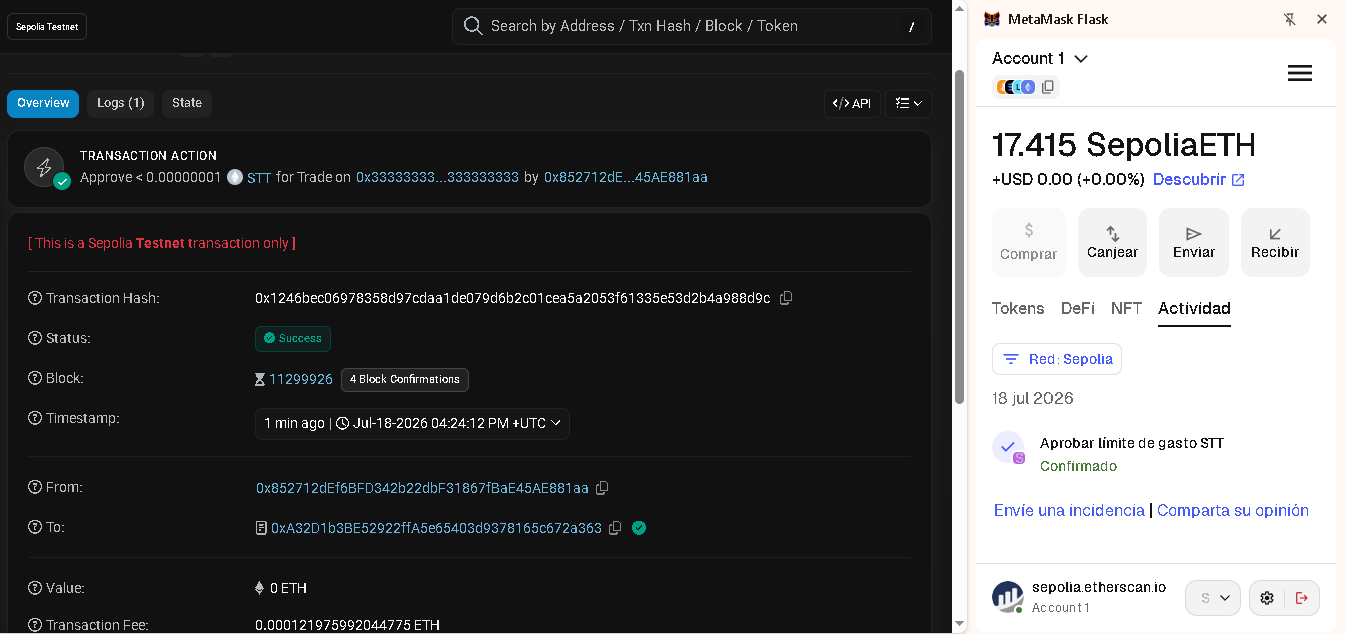
\includegraphics[width=\textwidth]{imgs/eval_scenario_g.png}
    \caption{Transacció confirmada a Sepolia i activitat corresponent a MetaMask}
    \label{fig:eval_scenario_g}
\end{figure}


\subsubsection{Escenari H -- Rendiment i comportament davant d’errors}

\noindent\textbf{Objectiu.} Mesurar el temps de resposta del flux complet i observar el comportament del sistema quan algun component local no està disponible.

\noindent\textbf{Requisits validats.} RNF1 i RNF3.

\noindent\textbf{Preparació.} Es realitzen diverses execucions representatives amb tots els serveis actius. Posteriorment, es repeteix la prova aturant temporalment Ollama o el backend local.

\noindent\textbf{Resultat esperat.} Amb tots els serveis actius, la resposta s’ha de generar en un temps compatible amb una interacció fluida. Davant d’un error, el sistema ha d’informar de la indisponibilitat del component sense bloquejar de manera injustificada la transacció.

\noindent\textbf{Resultat observat.} Amb Ollama actiu, els set casos van requerir entre 135,4 i 169,9 segons, amb una mitjana de 158,1 segons. En aturar Ollama, la primera prova va revelar que la generació de l'explicació no capturava l'error i provocava HTTP 500; el Snap va mostrar un fallback \texttt{DESCONOCIDO} sense bloquejar la cancel·lació. Després d'afegir una explicació local de reserva, la repetició va conservar el veredicte determinista \texttt{BAJO} i va completar el backend en 93 ms. Aquest resultat correspon al registre 48.

\noindent\textbf{Evidència.} Registre dels temps mesurats, captures de la interfície (Figura~\ref{fig:eval_scenario_h}), registres del backend i observació del comportament de MetaMask.

\begin{figure}[H]
    \centering
    \begin{subfigure}[t]{0.43\textwidth}
        \centering
        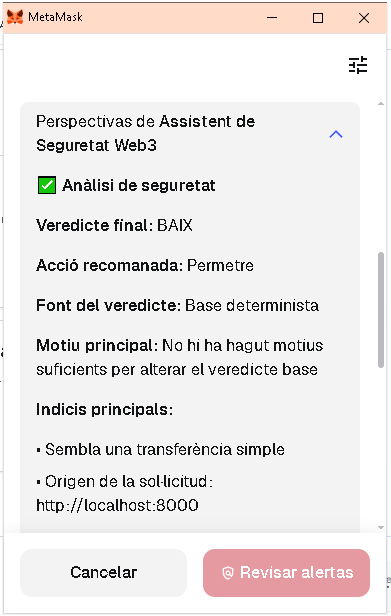
\includegraphics[width=\textwidth]{imgs/eval_scenario_h.png}
        \caption{Conservació del veredicte determinista}
    \end{subfigure}\hfill
    \begin{subfigure}[t]{0.43\textwidth}
        \centering
        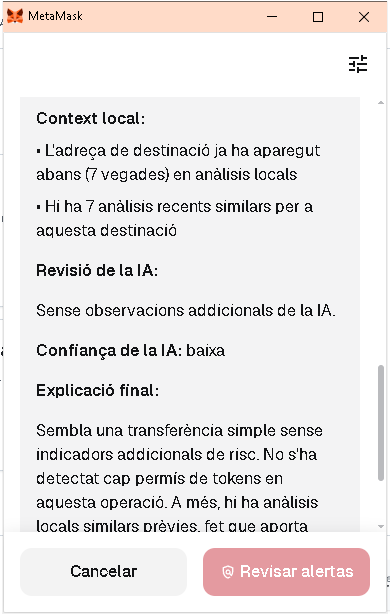
\includegraphics[width=\textwidth]{imgs/eval_scenario_h_detail.png}
        \caption{Explicació local sense observacions de la IA}
    \end{subfigure}
    \caption{Resposta determinista després d'aturar Ollama i aplicar el fallback local}
    \label{fig:eval_scenario_h}
\end{figure}

\clearpage
